
\begin{frame}[fragile]{What is RL?}

\begin{itemize}
\item An \textit{agent} interacts with an \textit{environment}. 
\begin{columns}
\begin{column}{0.5\textwidth}
    \begin{center}
     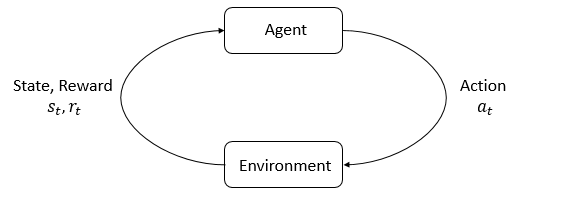
\includegraphics[width=\textwidth]{rl_diagram}
     \end{center}
\end{column}
\begin{column}{0.5\textwidth}  %%<--- here
\begin{lstlisting}[language=python]
  obs = env.reset()
  done = False
  while not(done):
  	act = agent.get_action(obs)
  	next_obs, reward, done, info = env.step(act)
  	obs = next_obs
\end{lstlisting}
\end{column}
\end{columns}
\item The goal of the agent is to maximize cumulative reward (called \textit{return}). 
\item The agent figures out how to attain its goal by trial and error.
\item Reinforcement learning (RL) is a field of study for algorithms that do that.
\end{itemize}

\end{frame}


\begin{frame}{Key Concepts in RL}

Before we can talk about algorithms, we have to talk about:
\begin{itemize}
\item Observation and action spaces
\item Policies
\item Trajectories
\item Reward and return
\item The RL optimization problem
\item Value and Action-Value Functions
\end{itemize}

\end{frame}

\begin{frame}{Observation and action spaces}

\begin{itemize}
\item A \textbf{state} is a complete-information description of the world
\item An \textbf{observation} is what the agent sees about the current state of the world
\item An environment is \textbf{fully observed} if the agent observes the whole state, otherwise \textbf{partially observed}
\item States, observations, and \textbf{actions} may be \textbf{continuous} or \textbf{discrete}
\end{itemize}

\begin{columns}
\begin{column}{0.5\textwidth}
\begin{center}
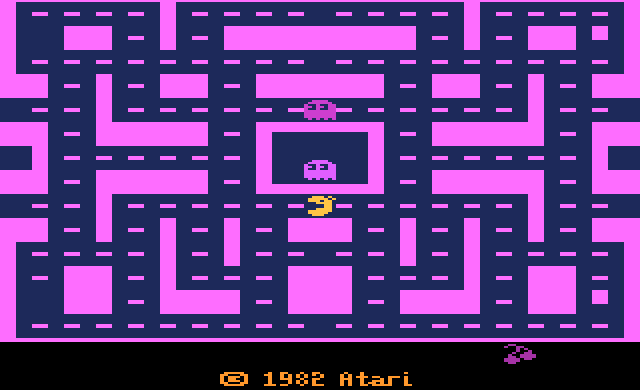
\includegraphics[width=0.9\textwidth]{ms_pacman}

Partially observed, continuous observation, discrete action
\end{center}
\end{column}
\begin{column}{0.5\textwidth}
\begin{center}
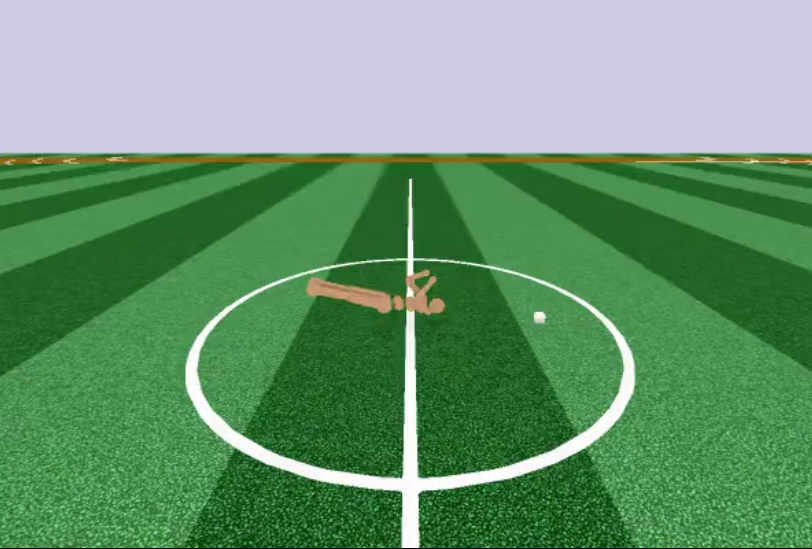
\includegraphics[width=0.9\textwidth]{knocked_down_standup}

Fully observed, continuous observation, continous action
\end{center}

\end{column}
\end{columns}

\end{frame}

\begin{frame}[fragile]{Policies}

A \textbf{policy} $\pi$ is a rule for selecting actions. It can be either
\begin{itemize}
\item \textbf{stochastic}, which means that it gives a probability distribution over actions, and actions are selected randomly based on that distribution ($a_t \sim \pi(\cdot|s_t)$),
\item or \textbf{deterministic}, which means that $\pi$ directly maps to an action ($a_t = \pi(s_t)$). 
\end{itemize}

\pause


\lstset{style=mystyle}

Examples of policies:
%
\begin{itemize}
\item Stochastic policy over discrete actions:
\begin{lstlisting}[language=python]
  obs = tf.placeholder(shape=(None, obs_dim), dtype=tf.float32)
  net = mlp(obs, hidden_dims=(64,64), activation=tf.tanh)
  logits = tf.layers.dense(net, units=num_actions, activation=None)
  actions = tf.squeeze(tf.multinomial(logits=logits,num_samples=1), axis=1)
\end{lstlisting}
\item Deterministic policy for a vector-valued continuous action:
\begin{lstlisting}[language=python]
  obs = tf.placeholder(shape=(None, obs_dim), dtype=tf.float32)
  net = mlp(obs, hidden_dims=(64,64), activation=tf.tanh)
  actions = tf.layers.dense(net, units=act_dim, activation=None)
\end{lstlisting}

\end{itemize}

\lstset{style=mystyle3}

\end{frame}


\begin{frame}{Trajectories}

\begin{itemize}
\item A \textbf{trajectory} $\tau$ is a sequence of states and actions in an environment:
\begin{equation*}
\tau = (s_0, a_0, s_1, a_1, ...).
\end{equation*}
\begin{itemize}
\item The initial state $s_0$ is sampled from a \textit{start state distribution} $\mu$:
%
\begin{equation*}
s_0 \sim \mu(\cdot).
\end{equation*}
\item State transitions depend only on the most recent state and action. They could be deterministic:
%
\begin{equation*}
s_{t+1} = f(s_t, a_t),
\end{equation*}
%
or stochastic:
%
\begin{equation*}
s_{t+1} \sim P(\cdot | s_t, a_t).
\end{equation*}
\end{itemize}
\item A trajectory is sometimes also called an \textbf{episode} or \textbf{rollout}. 
\end{itemize}

\end{frame}


\begin{frame}{Reward and Return}

The \textbf{reward} function of an environment measures how good state-action pairs are:
%
\begin{equation*}
r_t = R(s_t, a_t).
\end{equation*}

\begin{itemize}
\item Example: if you want a robot to run forwards but use minimal energy, $R(s, a) = v - \alpha \|a\|_2^2$. 
\end{itemize}
\pause
The \textbf{return} of a trajectory is a measure of cumulative reward along it. There are two main ways to compute return:
\begin{itemize}
\item Finite horizon undiscounted sum of rewards::
\begin{equation*}
R(\tau) = \sum_{t=0}^T r_t
\end{equation*}
\item Infinite horizon discounted sum of rewards:
\begin{equation*}
R(\tau) = \sum_{t=0}^{\infty} \gamma^t r_t
\end{equation*}
%
where $\gamma \in (0,1)$. This makes rewards less valuable if they are further in the future. (Why would we ever want this? Think about cash: it's valuable to have it sooner rather than later!)
\end{itemize}

\end{frame}

\begin{frame}{The Reinforcement Learning Problem}

In RL we want a policy which maximizes expected return. Thus the performance measure is
%
\begin{equation*}
J(\pi) = \underE{\tau \sim \pi}{R(\tau)},
\end{equation*}
%
and the \textbf{optimal policy} $\pi^*$ is:
%
\begin{equation*}
\pi^* = \arg \max_{\pi} J(\pi)
\end{equation*}

Note that by $\tau \sim \pi$, we mean
%
\begin{equation*}
s_0 \sim \mu(\cdot), \;\;\;\;\; a_t \sim \pi(\cdot|s_t), \;\;\;\;\; s_{t+1} \sim P(\cdot | s_t, a_t).
\end{equation*}

\end{frame}


\begin{frame}{Value Functions, Action-Value Functions, and Advantage Functions}

Value and action-value functions tell you the expected return after a state or state-action pair.
%
\begin{align*}
V^{\pi}(s) &= \underE{\tau \sim \pi}{R(\tau)\left| s_0 = s\right.} && \text{Start in }s\text{ and then sample from }\pi \\
Q^{\pi}(s,a) &= \underE{\tau \sim \pi}{R(\tau)\left| s_0 = s, a_0 = a\right.} && \text{Start in }s\text{, take action }a\text{, then sample from }\pi \\
V^*(s) &= \max_{\pi} \underE{\tau \sim \pi}{R(\tau)\left| s_0 = s\right.} && \text{Start in }s\text{ and then act optimally} \\
Q^*(s,a) &= \max_{\pi} \underE{\tau \sim \pi}{R(\tau)\left| s_0 = s, a_0 = a\right.} &&\text{Start in }s\text{, take action }a\text{, then act optimally}
\end{align*}

Value and action-value functions are connected:
%
\begin{align*}
V^{\pi}(s) &= \underE{a \sim \pi}{Q^{\pi}(s,a)}
\end{align*}

The advantage function for a policy tells you how much better or worse one action is than average:
%
\begin{align*}
A^{\pi}(s,a) &= Q^{\pi}(s,a) - V^{\pi}(s) 
\end{align*}

\end{frame}

\begin{frame}{Bellman Equations}

The value functions satisfy recursive \textbf{Bellman equations}:
%
\begin{align*}
V^{\pi}(s) &= \underE{a \sim \pi \\ s'\sim P}{r(s,a) + \gamma V^{\pi}(s')} \\
V^*(s) &= \max_a \underE{s'\sim P}{r(s,a) + \gamma V^*(s')} \\
Q^{\pi}(s,a) &= \underE{s'\sim P}{r(s,a) + \gamma \underE{a'\sim \pi}{Q^{\pi}(s',a')}} \\
Q^*(s,a) &= \underE{s'\sim P}{r(s,a) + \gamma \max_{a'} Q^*(s',a')}
\end{align*}

Basic idea: \textbf{The value of your starting point is the reward you expect to get from being there, plus the (discounted) value of wherever you land next.}

\vspace{2em}

Put another way: the cash you make in the rest of your life is the cash you make today plus all the cash you make for the rest of your life starting tomorrow

\end{frame}

%\begin{frame}{Operator Form of Bellman Equations}
%
%In operator form, where $\calT_v : V \to V$ and $\calT_q: Q\to Q$,
%%
%\begin{align*}
%V^{\pi} &= \calT^{\pi}_v V^{\pi} \\
%V^* &= \calT^*_v V^* \\
%Q^{\pi} &= \calT^{\pi}_q Q^{\pi} \\
%Q^* &= \calT^*_q Q^*
%\end{align*}
%\end{frame}

\begin{frame}{$Q^*$}
The optimal $Q$ function, $Q^*$, is especially important because it gives us a policy. In any state $s$, the optimal action is
%
\begin{equation*}
a^* = \arg \max_a Q^* (s, a).
\end{equation*}

We can measure how good a $Q^*$-approximator, $Q_{\theta}$, is by measuring its \textbf{mean-squared Bellman error}:
%
\begin{equation*}
\ell(\theta) = \frac{1}{|\calD|} \sum_{(s,a,s',r) \in \calD} \left( Q_{\theta}(s,a) - \left(r + \gamma \max_{a'} Q_{\theta}(s',a')\right)\right)^2.
\end{equation*}
%
This (roughly) says how well it satisfies the Bellman equation
%
\begin{equation*}
Q^*(s,a) = \underE{s'\sim P}{r(s,a) + \gamma \max_{a'} Q^* (s',a')}
\end{equation*}

\end{frame}